To estimate the feasibility of making a measurement of the 21cm-\lya cross-power
spectrum, it is important to define the sources of error

\begin{equation}
\sigma_{21} \left(k \right) = \left[ P_{21} \left(k \right) + P_{21, \textrm{N}} \left(k \right) \right]
\end{equation}

\begin{equation}
P_{21, \textrm{N}} = X^2 Y \frac{T^2_{\textrm{sys}}}{2 t} \frac{\Omega_{\textrm{p}}^2}{\Omega_{\textrm{pp}}}
\end{equation}

\begin{table}[]
\caption{Observing parameters for uncertainty calculations}
\centering
\begin{tabular}{cc}
\hline
\multicolumn{2}{c}{HERA Observing Parameters}                                                                                                                \\ \hline
\multicolumn{1}{c|}{Observing Days}                                                         & 180                                                            \\
\multicolumn{1}{c|}{Time Per Day (hrs)}                                                     & 6                                                              \\
\multicolumn{1}{c|}{Bandwidth (MHz)}                                                        & 8                                                              \\
\multicolumn{1}{c|}{Dish Size (m)}                                                          & 14                                                             \\
\multicolumn{1}{c|}{Number of Elements}                                                     & 320                                                            \\
\multicolumn{1}{c|}{$T_{\rm sys}$}                                                          & $100 + 120 \left( \nu / 150 \, \textrm{MHz} \right)^{-2.55}$ K \\ \hline
\multicolumn{2}{c}{SPHEREx Observing Parameters}                                                                                                             \\ \hline
\multicolumn{1}{c|}{$x_{\rm pix} \left( '' \right)$}                                        & 6.2                                                            \\
\multicolumn{1}{c|}{$\sigma_{\rm N} \left[ \rm erg \, s^{-1} \, cm^{-2} \, sr^{-1}\right]$} & $3 \times 10^{-20}$                                            \\
\multicolumn{1}{c|}{$V_{\rm vox} \left(\textrm{Mpc}^{3} \right)$}                                         & 0.3                                                            \\
\multicolumn{1}{c|}{$\textrm{R}_{\rm res}$}                                                 & 41.5                                                           \\ \hline
\end{tabular}
\end{table}

\lya uncertainty

\begin{equation}
  \sigma_{\rm Ly\alpha} = \left[ P_{\rm Ly\alpha} + P_{\textrm{Ly}\alpha, \textrm{N}} \right]
\end{equation}

\begin{equation}
P_{\textrm{Ly}\alpha, \textrm{N}} = \sigma_{\rm N}^2 V_{\text{vox}} \textrm{W}_{\rm Ly\alpha}\left(k_{\perp}, k_{\parallel}\right)
\end{equation}

\begin{equation}
  \textrm{W}_{\rm Ly\alpha}\left( k_{\perp}, k_{\parallel} \right) = \exp \left(\left( k_{\perp} / k_{\perp, \textrm{res}}\right)^2 + \left( k_{\parallel} / k_{\parallel, \textrm{res}}\right)^2\right)
\end{equation}


$V_{\rm vox} = A_{\rm pix} r_{\rm pix}$

21cm-\lya uncertainty


\begin{equation}
    \sigma^2_{21, \rm Ly\alpha} = \frac{1}{2} \left[ P^2_{21, \rm Ly\alpha} + \sigma_{21} \sigma_{\rm Ly\alpha} \right]
\end{equation}

\begin{figure}[th]
	\centering
	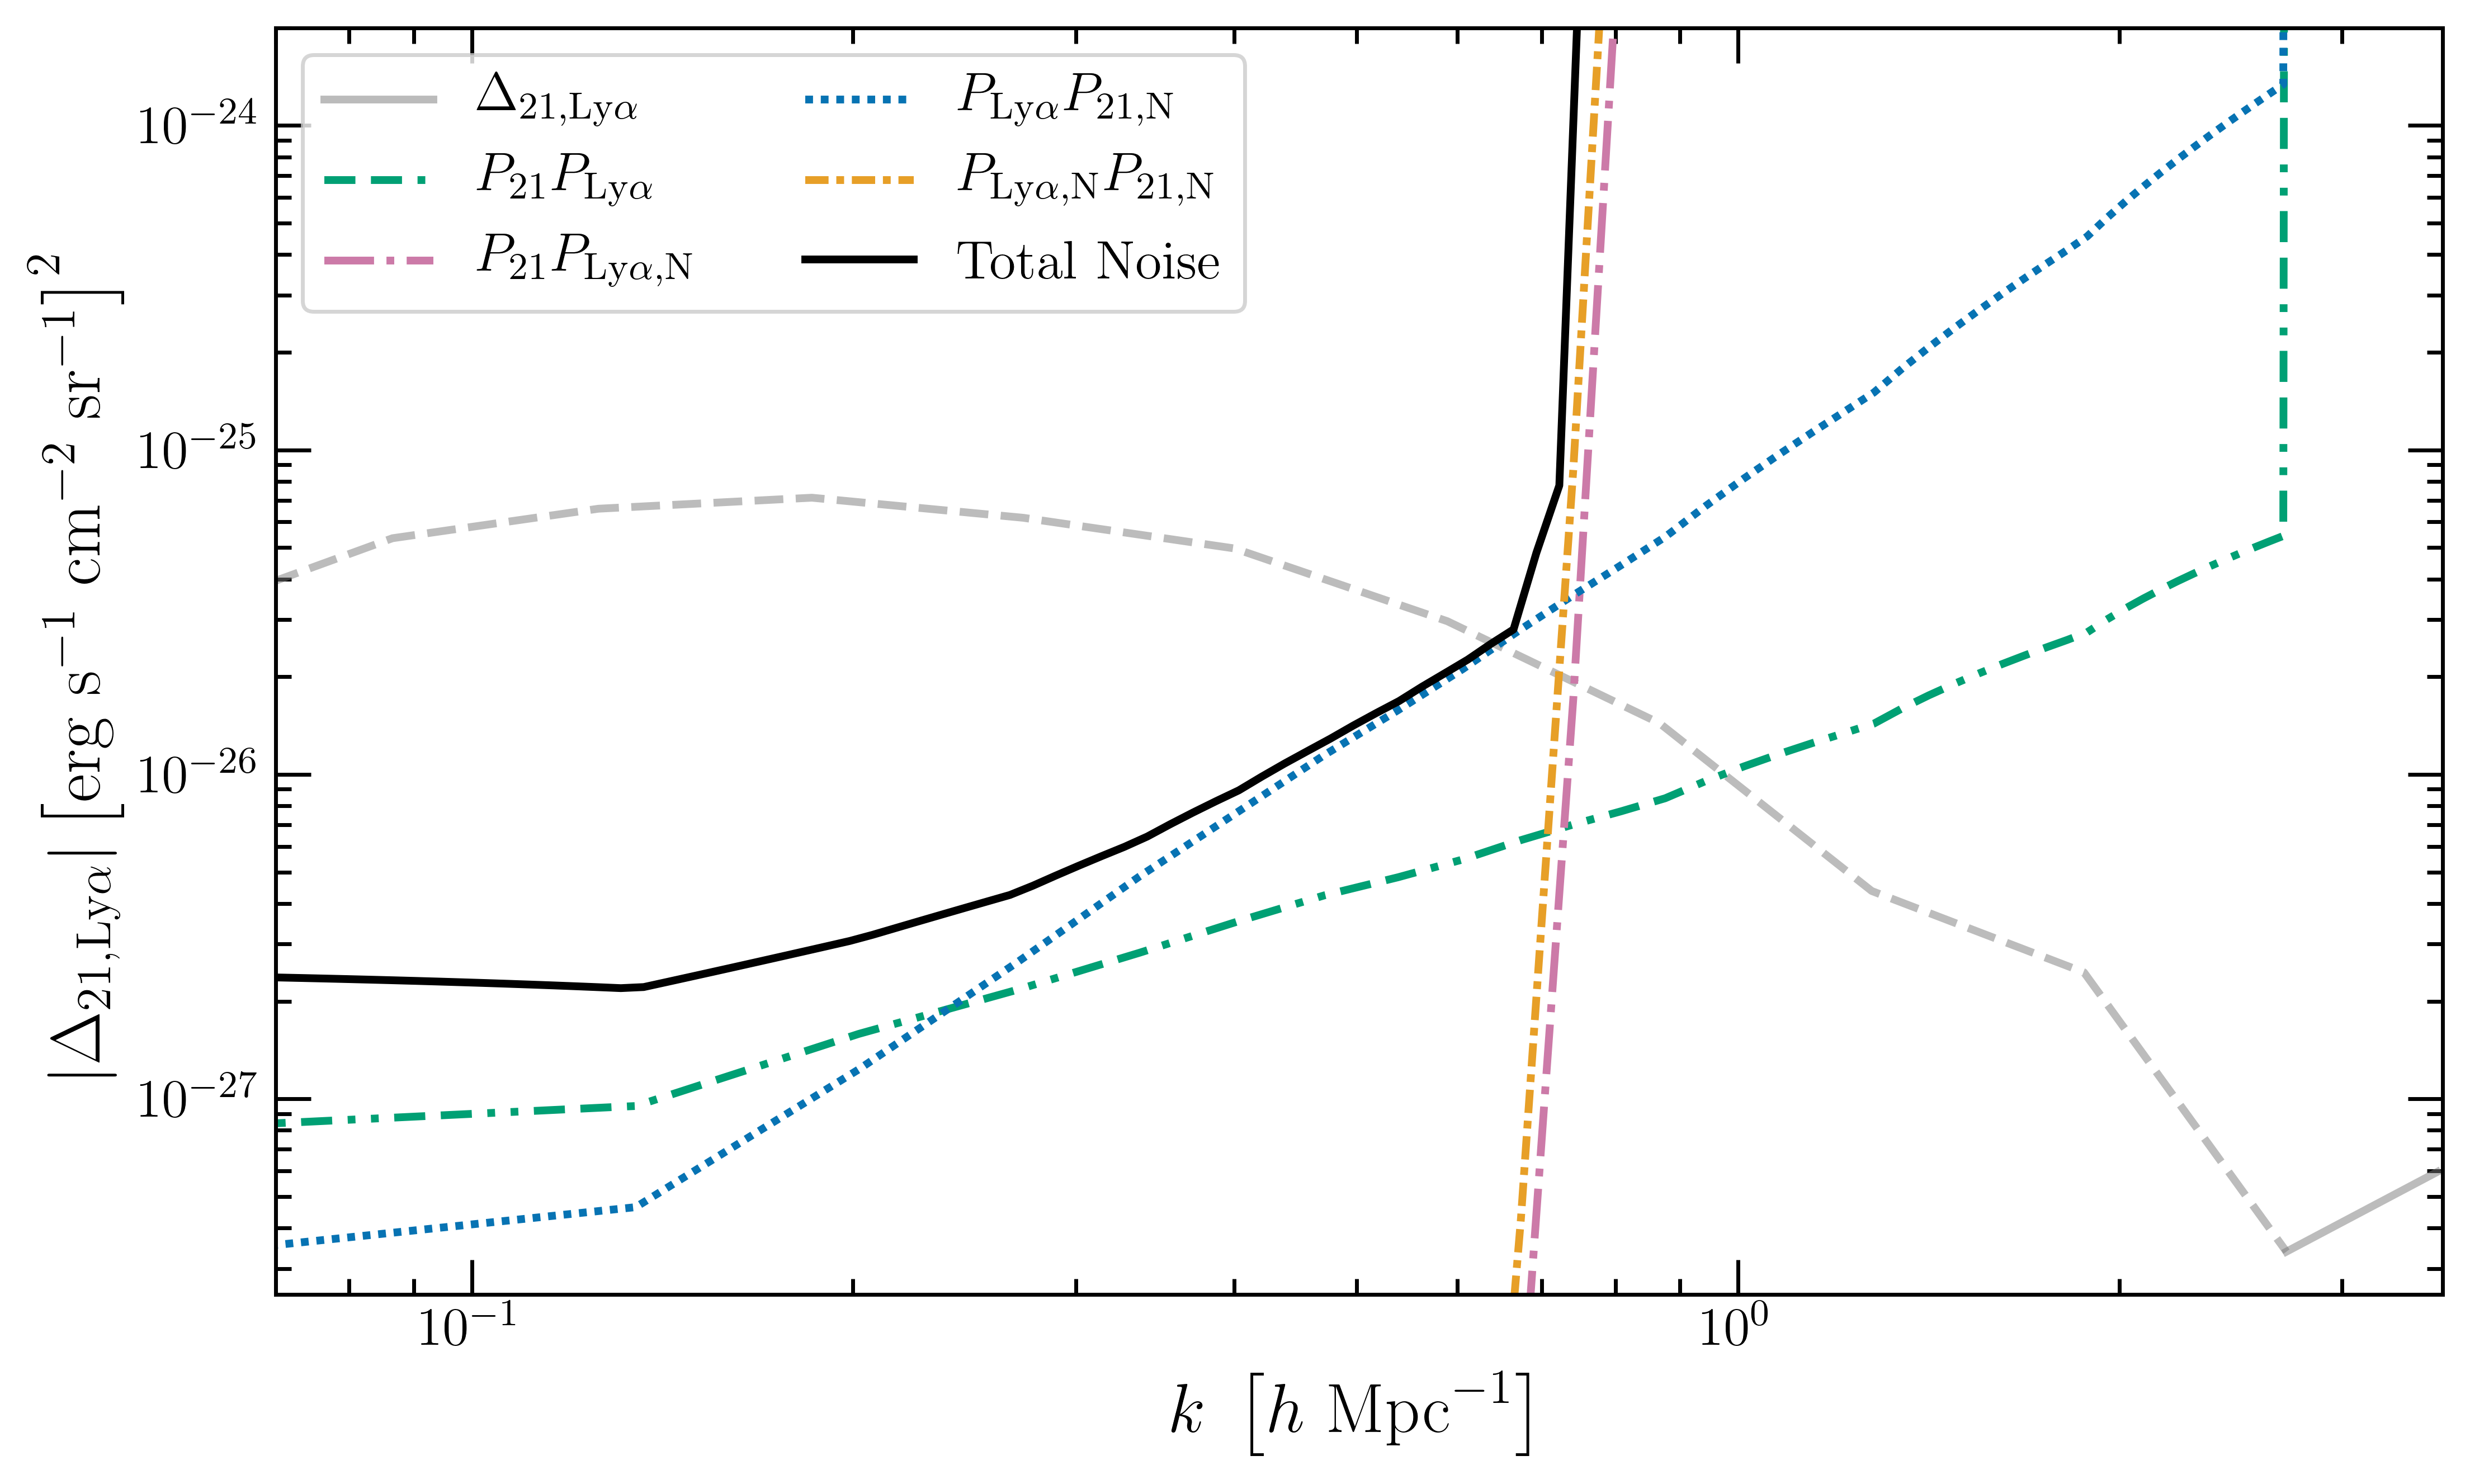
\includegraphics[width=0.95\textwidth]{error_budget.png}
	\caption[Cross-Power Spectrum Error Budget]{Error budgets of the sensitivity on the cross-power spectrum as measured by HERA and SPHEREx
  at $z = 8$. The terms $P_{21, \textrm{N}}$ and $P_{\textrm{Ly}\alpha, \textrm{N}}$ represent the thermal noise variance from HERA and SPHEREx respectively. Here, I neglect plotting the cross-power sample variance term, $P_{21, \textrm{Ly}\alpha }$ as its contribution is neglible, however, it is represented in the total noise of the measurement. For reference, the cross-power spectrum is plotted in gray.}
	\label{fig:error_budget}
\end{figure}
